\documentclass[14pt, aspectratio=169, handout]{beamer}
\usetheme{Copenhagen}
\usecolortheme{seahorse}
\setbeamertemplate{navigation symbols}{}
\setbeamertemplate{headline}{}

%\usepackage{pgfpages}
%\pgfpagesuselayout{4 on 1}[a4paper, border shrink=5mm]

\usepackage{graphicx} % Required for inserting images
\usepackage{multicol}
%\usepackage{enumitem}
\usepackage{amsfonts}
\usepackage{amsmath}
\usepackage{xcolor}
\definecolor{myblue}{RGB}{0, 0, 255} 
\definecolor{mygreen}{RGB}{0, 180, 80}
\definecolor{myred}{RGB}{153, 0, 0}
\definecolor{myorange}{RGB}{255, 153, 51}
\definecolor{mypurple}{RGB}{102, 0, 204}
\usepackage{tikz}

%--- commands for transform arrows----------------
\newcommand{\transform}[2]{%
    \begin{tikzpicture}
        % Open circle
        \draw[thick] (0,0) circle (0.1);
        % Line with number above and adjustable length
        \draw[thick] (0.1,0) -- (#2,0) node[midway, above] {#1};
        % Filled circle
        \filldraw[thick] (#2,0) circle (0.1);
    \end{tikzpicture}%
}
\newcommand{\invtransform}[2]{%
    \begin{tikzpicture}
        % filled circle
        \filldraw[thick] (0,0) circle (0.1);
        % Line with number above and adjustable length
        \draw[thick] (0.1,0) -- (#2 -0.1,0) node[midway, above] {#1};
        % open circle
        \draw[thick] (#2,0) circle (0.1);
    \end{tikzpicture}%
}
\newcommand{\verticaltransform}[4]{%
    \begin{tikzpicture}
        % Open circle at the bottom with text below
        \filldraw[thick] (0,0) circle (0.1) node[below=3pt] {$#4$};
        % Vertical line with number on the left
        \draw[thick] (0,0.1) -- (0,#2 -0.1) node[midway, left] {#1};
        % Filled circle at the top with text above
        \draw[thick] (0,#2) circle (0.1) node[above=3pt] {$#3$};
    \end{tikzpicture}%
}
\newcommand{\verticalinvtransform}[4]{%
    \begin{tikzpicture}
        % Open circle at the bottom with text below
        \draw[thick] (0,0) circle (0.1) node[below=3pt] {$#4$};
        % Vertical line with number on the left
        \draw[thick] (0,0.1) -- (0,#2) node[midway, left] {#1};
        % Filled circle at the top with text above
        \filldraw[thick] (0,#2) circle (0.1) node[above=3pt] {$#3$};
    \end{tikzpicture}%
}

\definecolor{darkblue}{RGB}{0, 0, 139}
\definecolor{lightblue}{RGB}{173, 216, 230}

\title{SST1 Übungsstunde 9}
\author{Matteo Dietz}
\date{November 2024}

\begin{document}

\maketitle

\begin{frame}{Themenüberblick}
    \begin{itemize}
        \item \textbf{Repetition: Abtasttheorem}
        \item \textbf{Zeitdiskrete Signale und Systeme}
        \item[] Zeitdiskrete Fouriertransformation (DTFT)
        \item[] Zeitdiskrete LTI-Systeme und Systemeigenschaften
        \item[] Differenzengleichungen
    \end{itemize}
\end{frame}


\begin{frame}{Aufgaben für diese Woche}
    \begin{itemize}
        \item[] \textbf{97}, 98, 99, 100, 101, \textbf{102}, \textbf{103}, \textbf{104}, 105, 106, \textbf{107}, \textbf{108}, 109, \textbf{110}, \textbf{111}, \textbf{112}, 113
        \item[] 
        \item[] Die \textbf{fettgedruckten} Übungen empfehle ich, weil sie wesentlich zu eurem Verständnis der Theorie beitragen und/oder sehr prüfungsrelevant sind.
    \end{itemize}
\end{frame}


\begin{frame}{Abgetastete Signale im Frequenzbereich}
    \begin{center}
        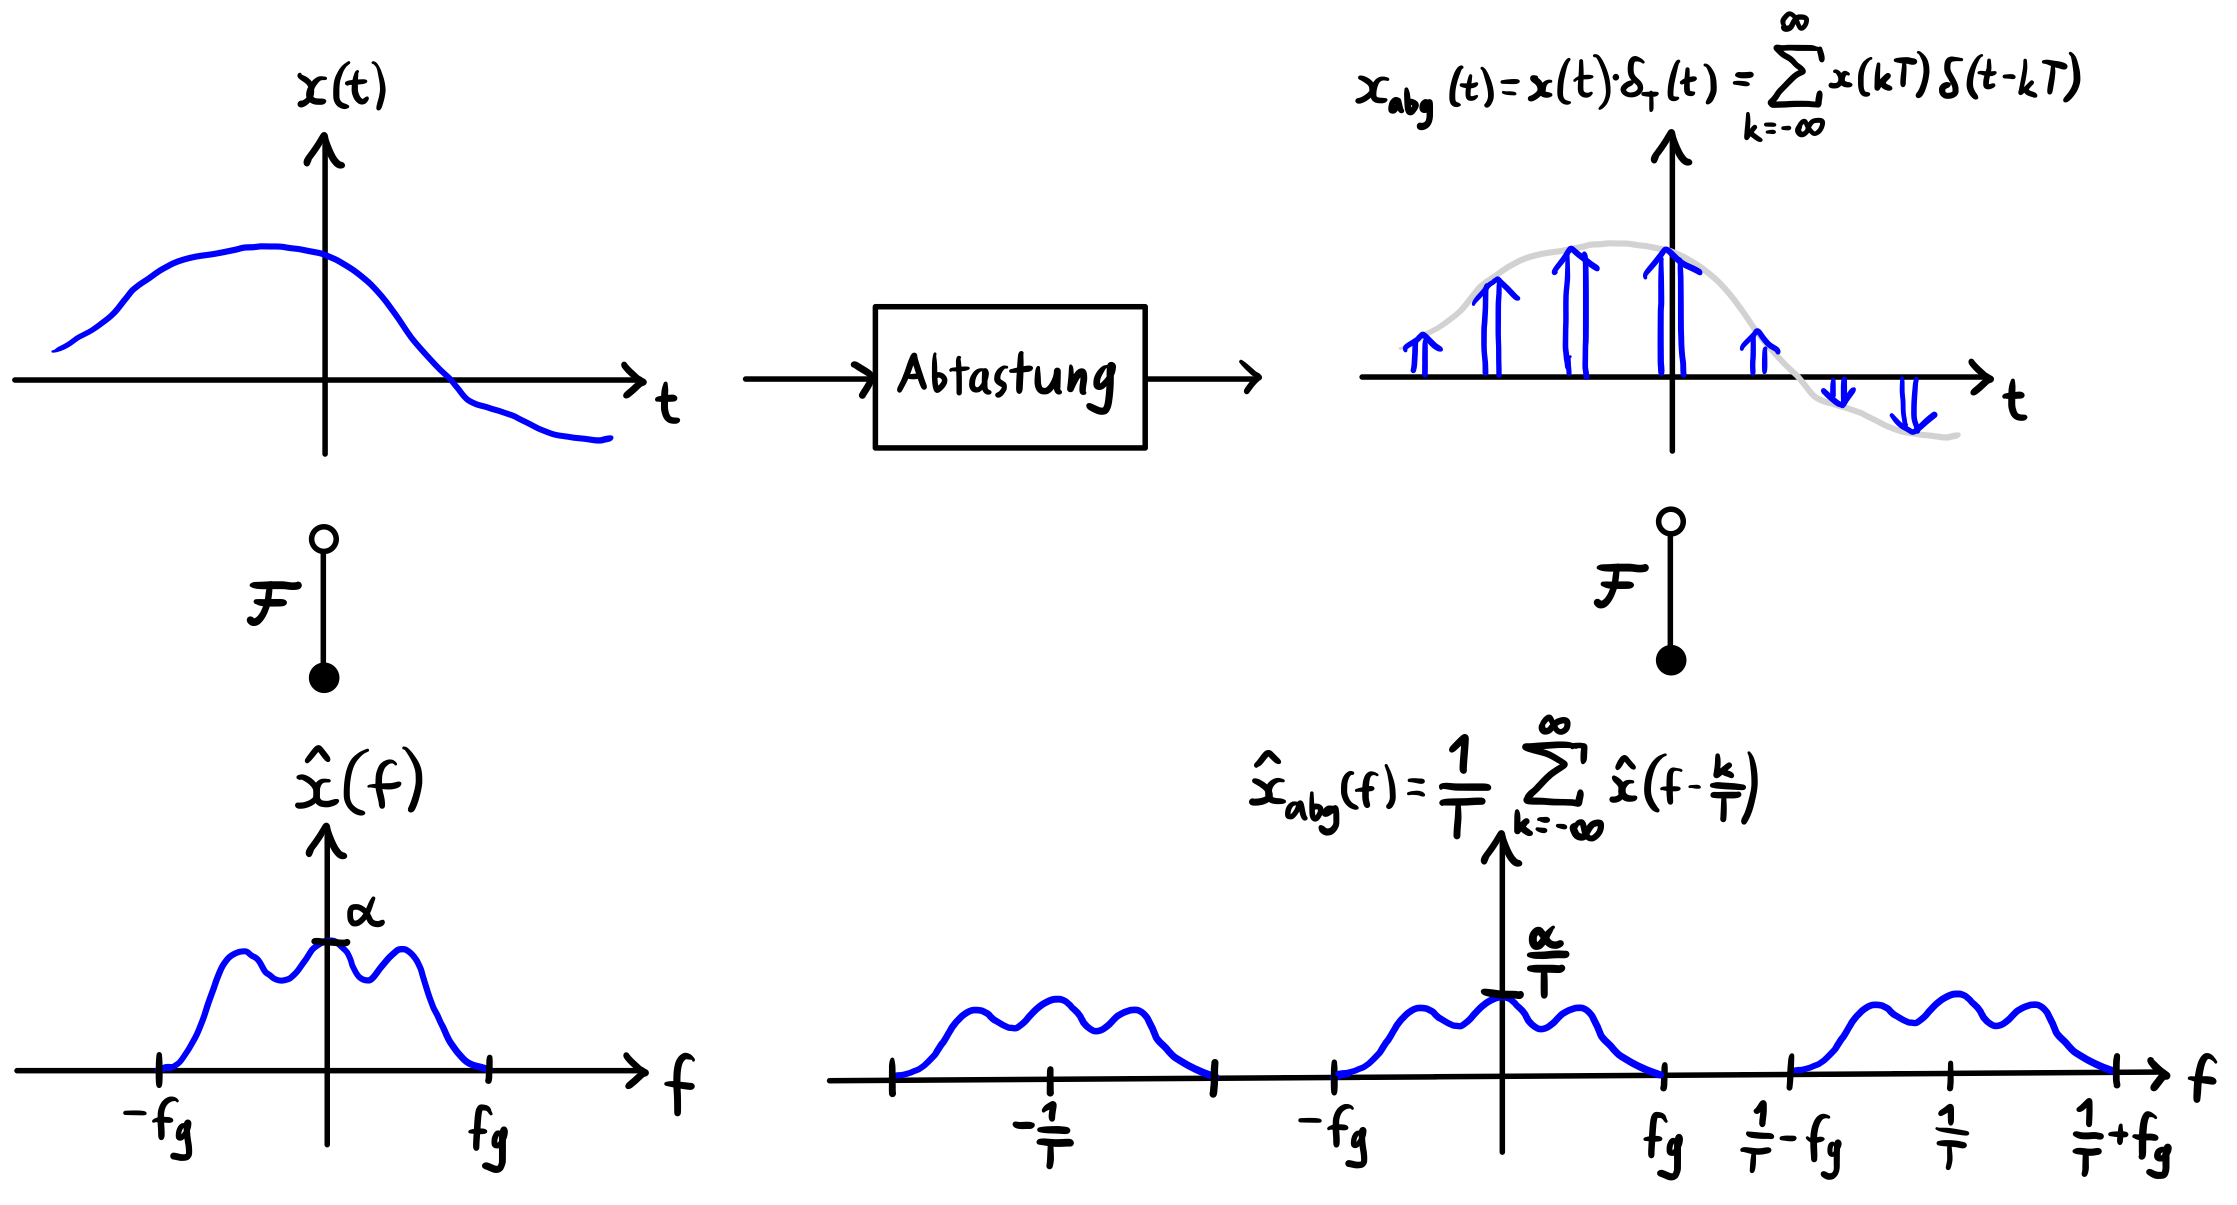
\includegraphics[width=0.92\linewidth]{figures/abtastung2.jpg}
    \end{center}
\end{frame}

\begin{frame}{Abgetastete Signale im Frequenzbereich}
\vspace*{-0.5cm}
\begin{align*}
    x_{abg.}(t) = x(t)\delta_T(t) &= \sum_{k=-\infty}^{\infty} x(kT)\delta(t-kT) \\
    \transform{20.}{2} \hspace{10pt} \hat{x}_{abg.}(f) &= \frac{1}{T} \sum_{k = -\infty}^\infty \hat{x}\left( f- \frac{k}{T} \right)
\end{align*}
    \fcolorbox{darkblue}{lightblue}{%
    \parbox{\dimexpr\linewidth-2\fboxsep-2\fboxrule\relax}{
        \vspace{0.25cm}
        Die \textbf{Abtastung im Zeitbereich} entspricht einer \textbf{Periodisierung im Frequenzbereich}. (Die Kopien sind um Faktor $\frac{1}{T}$ skaliert.)
        \vspace{0.25cm}
    }}%
    \vspace*{12pt}
    \begin{itemize}
        \item $f_g$ ist die Bandbreite von $x(t)$, $f_s := \displaystyle\frac{1}{T}$ ist die Abtastfrequenz
    \end{itemize}
\end{frame}

\begin{frame}{1. \textcolor{myblue}{\textbf{Kritische Abtastung: $f_s = 2 f_g$}}}
    \begin{center}
        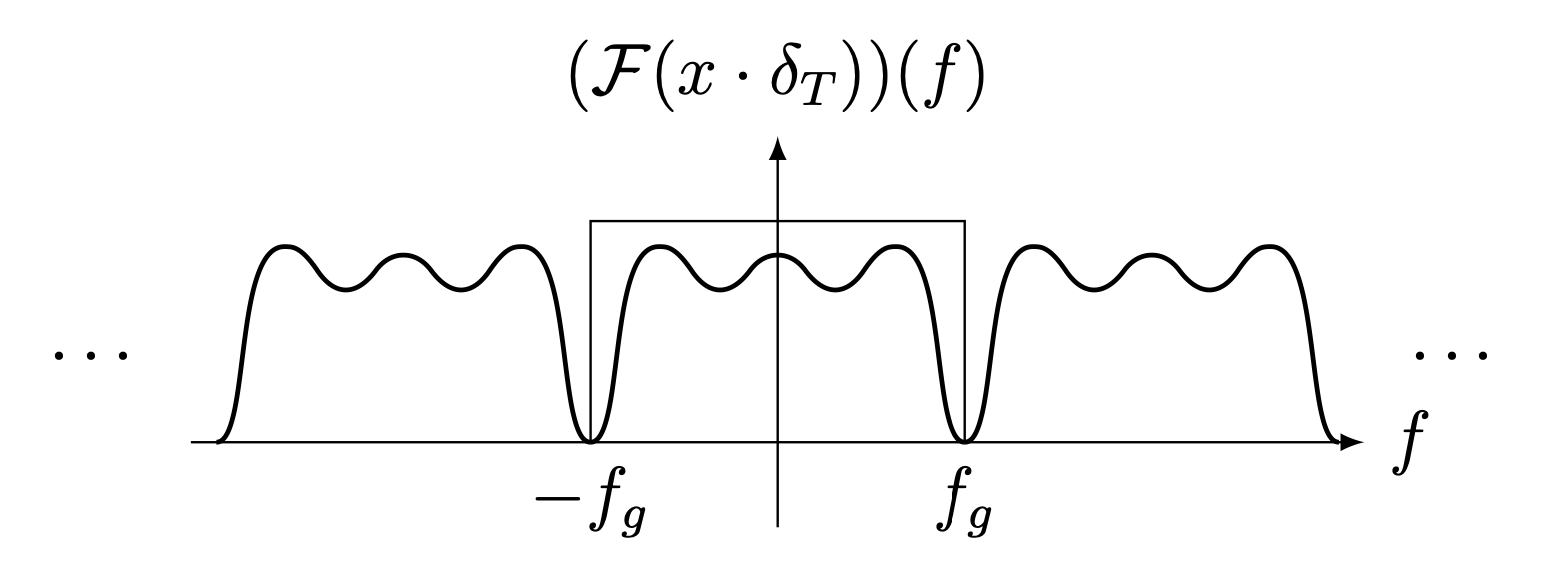
\includegraphics[width=0.85\linewidth]{figures/krit_abtast.png}
    \end{center}
    $\implies$ Wir können das Signal mit einem idealen Tiefpassfilter der Breite $W = f_g$ rekonstruieren

\end{frame}

\begin{frame}{2. \textcolor{myblue}{\textbf{Überabtastung: $f_s > 2f_g$}}}
    \begin{center}
        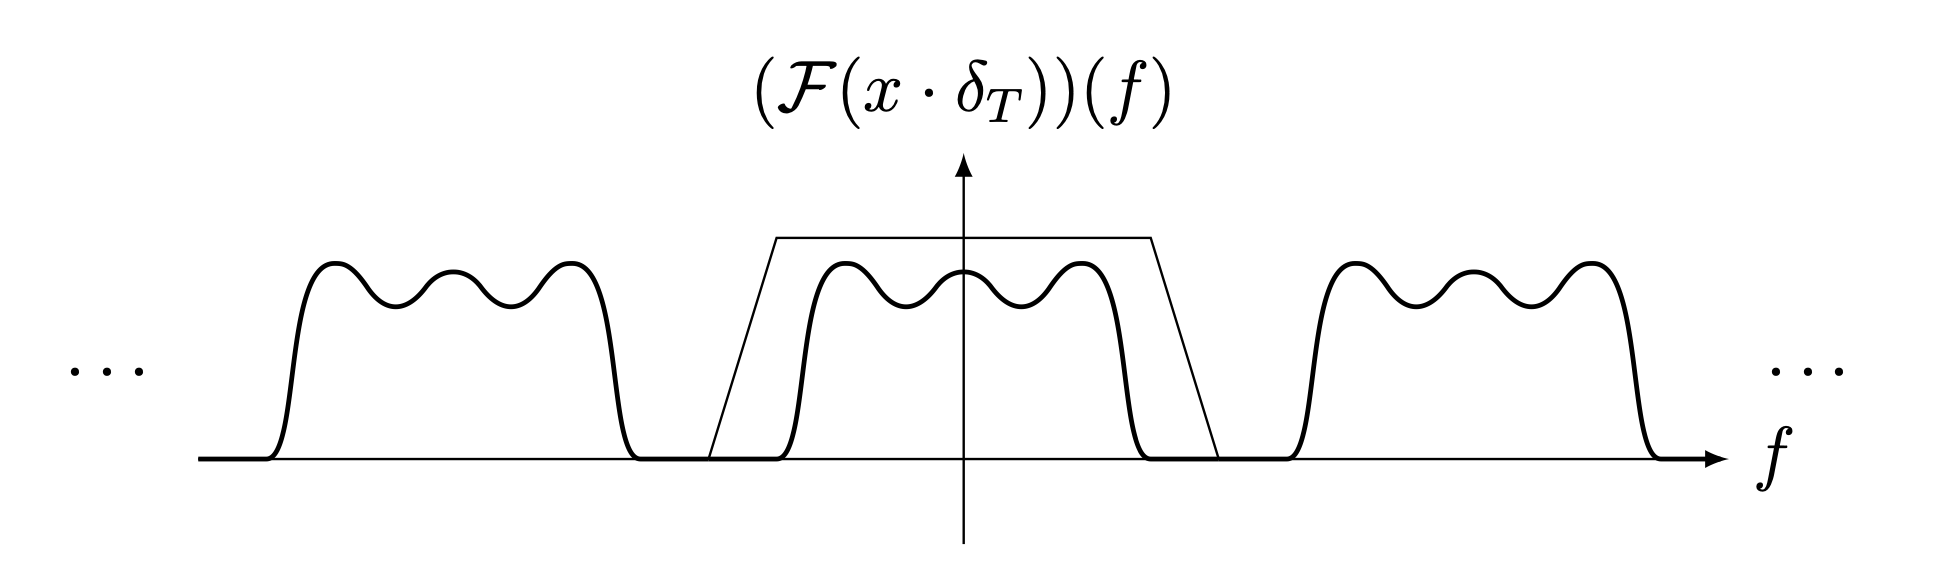
\includegraphics[width=0.85\linewidth]{figures/ueberabtast.png}
    \end{center}

\textbf{Vorteile an Überabtastung:}
\begin{enumerate}
    \item Wir können einen stabilen Tiefpassfilter verwenden.
    \item Überabtastung verringert die Empfindlichkeit auf Rauschen.
\end{enumerate}
\end{frame}

\begin{frame}{3. \textcolor{myblue}{\textbf{Unterabtastung: $f_s < 2 f_g$}}}
    \begin{center}
        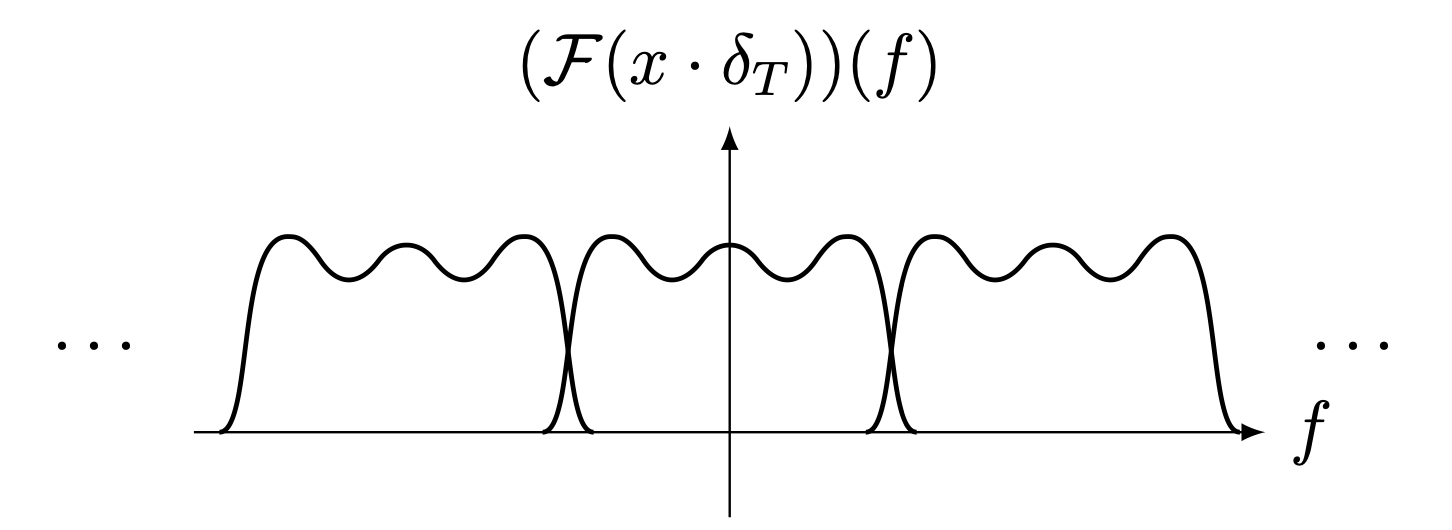
\includegraphics[width=0.8\linewidth]{figures/aliasing1.png}
    \end{center}
    Es gibt \textbf{Aliasing}. Mit Hilfe eines Tiefpassfilters erhalten wir keine perfekte Version von $\hat{x}(f)$.
\end{frame}

\begin{frame}{\textcolor{myblue}{\textbf{Abtasttheorem}}}
    \fcolorbox{darkblue}{lightblue}{%
    \parbox{\dimexpr\linewidth-2\fboxsep-2\fboxrule\relax}{
        \vspace*{0.25cm}
        Ein Signal mit der Bandbreite $f_g$ kann aus seinen Abtastwerten, genommen mit einer Rate von $f_s \geq 2f_g$, eindeutig rekonstruiert werden.\\
        Die kritische Rate $f_s = 2 f_g$ wird als \textbf{Nyquistrate} bezeichnet.
        \vspace*{0.25cm}
    }}%
\end{frame}

\begin{frame}{Rekonstruktion}
    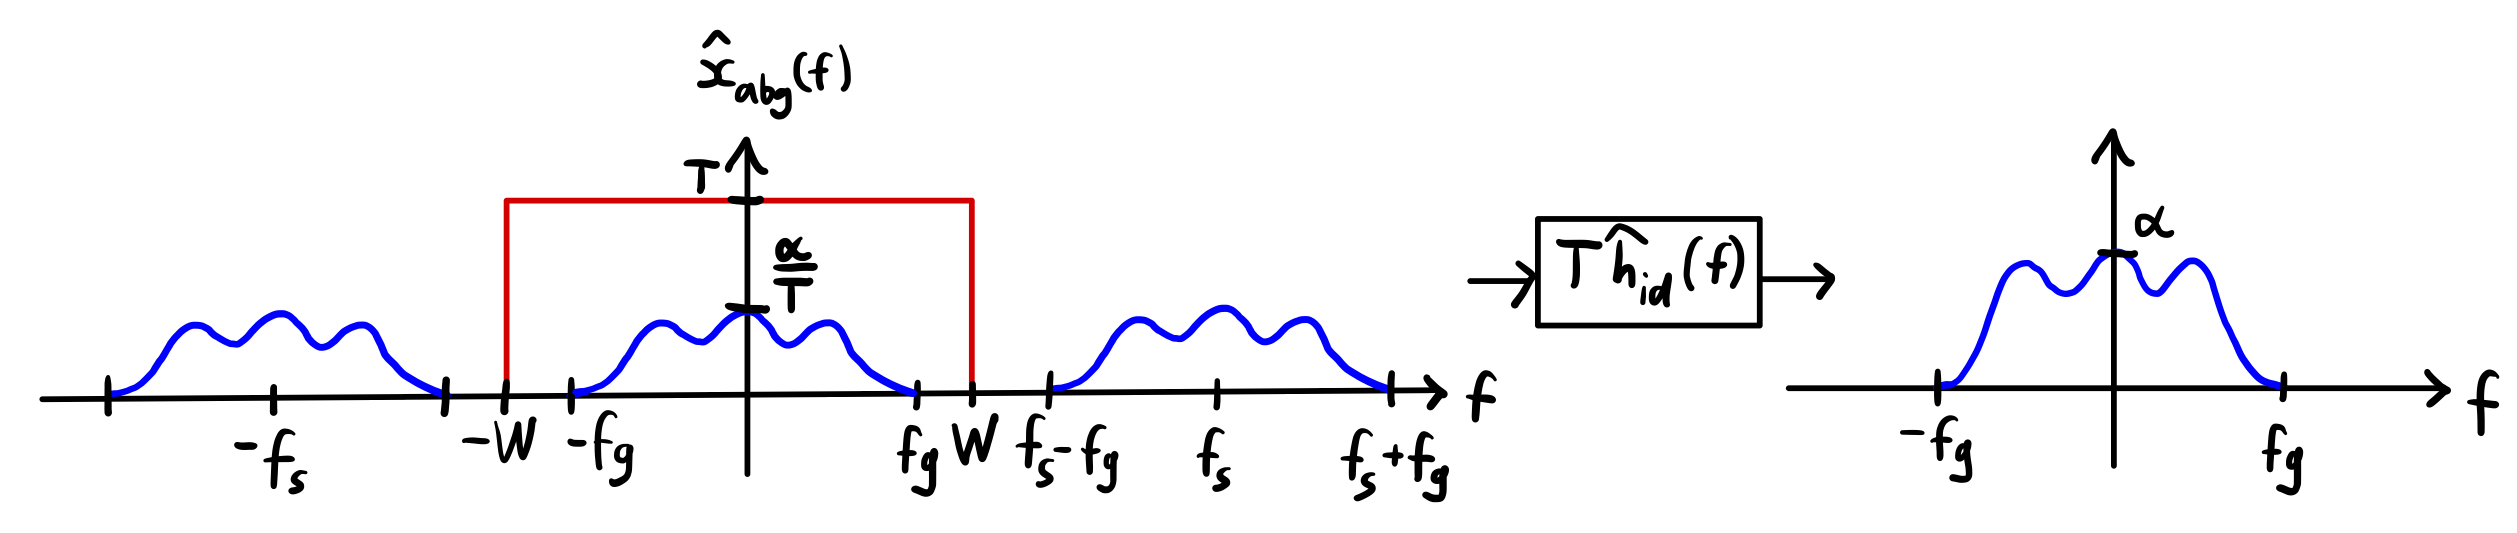
\includegraphics[width=\linewidth]{figures/filtering1.jpg}
\end{frame}


\begin{frame}{Rekonstruktion}
\vspace*{-0.5cm}
    \begin{itemize}
    \item[] 
    \item Allgemeine Rekonstruktion eines Signals aus Abtastwerten:
    \item[] 
    \fcolorbox{darkblue}{lightblue}{%
    \parbox{\dimexpr\linewidth-2\fboxsep-2\fboxrule\relax}{
       $$y(t) = T \displaystyle\sum_{k = -\infty}^\infty x(kT)h(t-kT)$$
    }}%
    \item[] 
    \item[] 
    \item Kritische Abtastung $\implies$ idealer Tiefpassfilter mit Breite $W = f_g = \frac{f_s}{2} = \frac{1}{2T} \implies \hat{h}_{id}(f) \hspace{8pt}\invtransform{}{1} \hspace{8pt} h_{id}(t)=\displaystyle\frac{\sin(2 \pi W t)}{\pi t}$
    \item[] 
    \item[] $\implies y(t) = x(t) = \displaystyle\sum_{k=-\infty}^\infty x(kT)\displaystyle\frac{\sin\left(\frac{\pi}{T}(t-kT)\right)}{\frac{\pi}{T}(t-kT)}$
\end{itemize}
\end{frame}

\begin{frame}{Zeitdiskrete Signale}
    Abtastung im Zeitbereich $\implies$ periodische Fortsetzung des Spektrums:
$$\hat{x}_{\text{abg}}(f) = \mathcal{F}\{x \cdot \delta_T\}(f) = \frac{1}{T}\sum_{k=-\infty}^{\infty}\hat{x}\left( f- \frac{k}{T} \right)$$
Dieses Signal ist $\frac{1}{T}-$periodisch und besitzt somit eine Fourierreihendarstellung.
\end{frame}

\begin{frame}{Poisson \& Dualität}
    \textbf{Poissonsche Summenformel}
    $$\sum_{k=-\infty}^\infty h(t + kT) = \frac{1}{T} \sum_{k=-\infty}^\infty \hat{h}(k/T)e^{2 \pi i k t/T}$$
    \textbf{Dualität der Fouriertransformation}
    \begin{center}
        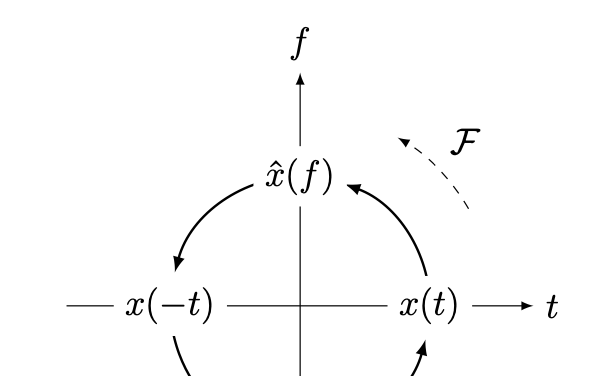
\includegraphics[width=0.4\textwidth]{figures/dualitaet_1.png}
    \end{center}
\end{frame}

\begin{frame}{Zeitdiskrete Signale im Frequenzbereich}
    \begin{align*}
        \hat{x}_{\text{abg}}(f) &= \frac{1}{T}\sum_{k=-\infty}^{\infty}\hat{x}\left( f- \frac{k}{T} \right) = \frac{1}{T}\cdot T \sum_{k=-\infty}^{\infty} \underbrace{\hat{\hat{x}}(kT)}_{x(-kt)}e^{2 \pi i k f T} \\
        &= \sum_{k=-\infty}^\infty x(-kT)e^{2 \pi i k f T} = \sum_{k=-\infty}^\infty \underbrace{x(kT)}_{x_d[k]=c_k}e^{-2 \pi i k f T}
    \end{align*}
$\implies$ Darstellung als komplexe Fourierreihe: \textbf{Abtastwerte} $x(kT)$ sind die Koeffizienten der Fourierreihe des Spektrums $\hat{x}_{\text{abg}}(f)$.
\end{frame}

\begin{frame}{Zeitdiskrete Signale im Frequenzbereich}
    Wir definieren $\theta = Tf$ und erhalten mithilfe der Formel von oben
    \begin{align*}
        \sum_{k=-\infty}^\infty x_d[k] e^{-2\pi i k \theta} &= \sum_{k=-\infty}^\infty x(kT) e^{-2\pi i k T f} \\
        &= \frac{1}{T}\sum_{k=-\infty}^{\infty}\hat{x}\left( f- \frac{k}{T} \right) \\
        &= \frac{1}{T}\sum_{k=-\infty}^{\infty}\hat{x}\left( \frac{\theta - k}{T} \right) = \hat{x}_d(\theta)
    \end{align*}
\end{frame}

\begin{frame}{\textcolor{blue}{\textit{Discrete Time Fourier Transform}} (DTFT)}
    \fcolorbox{darkblue}{lightblue}{%
    \parbox{\dimexpr\linewidth-2\fboxsep-2\fboxrule\relax}{\begin{itemize}
        \item[] $(\textbf{DTFT}) \hspace{50pt} \hat{x}_d(\theta) = \displaystyle\sum_{n=-\infty}^\infty x_d[n]e^{-2 \pi i n \theta}$
        \item[] $(\textbf{IDTFT}) \hspace{46pt} x_d[n]=\displaystyle\int_0^1 \hat{x}_d(\theta)e^{2 \pi i n \theta} \text{d}\theta$
    \end{itemize}
}}%
\end{frame}

\begin{frame}{Rücktransformation}

\end{frame}

\begin{frame}{DTFT: Bemerkungen}
    \begin{itemize}
    \item diskreter Zeitbereich $ \transform{\text{DTFT}}{1.5}$ kontinuierlicher Frequenzbereich
    \item[] 
    \item $\theta = Tf = \frac{f}{f_s}$ ist die \textbf{relative Frequenz}
    \item[] ($T=$ Abtastperiode und $f_s=$ Abtastfrequenz)
    \item[] 
    \item $\hat{x}_d(\theta) = \displaystyle\frac{1}{T} \sum_{k=-\infty}^\infty \hat{x}\left( \frac{\theta - k}{T} \right)$ ist \textbf{1-periodisch} in $\theta$.
\end{itemize}
\end{frame}

\begin{frame}{DTFT: Bemerkungen}
\begin{itemize}
    \item $\hat{x}_d(\theta) = \displaystyle\frac{1}{T} \sum_{k=-\infty}^\infty \hat{x}\left( \frac{\theta - k}{T} \right)$ ist \textbf{1-periodisch} in $\theta$.
\end{itemize}
    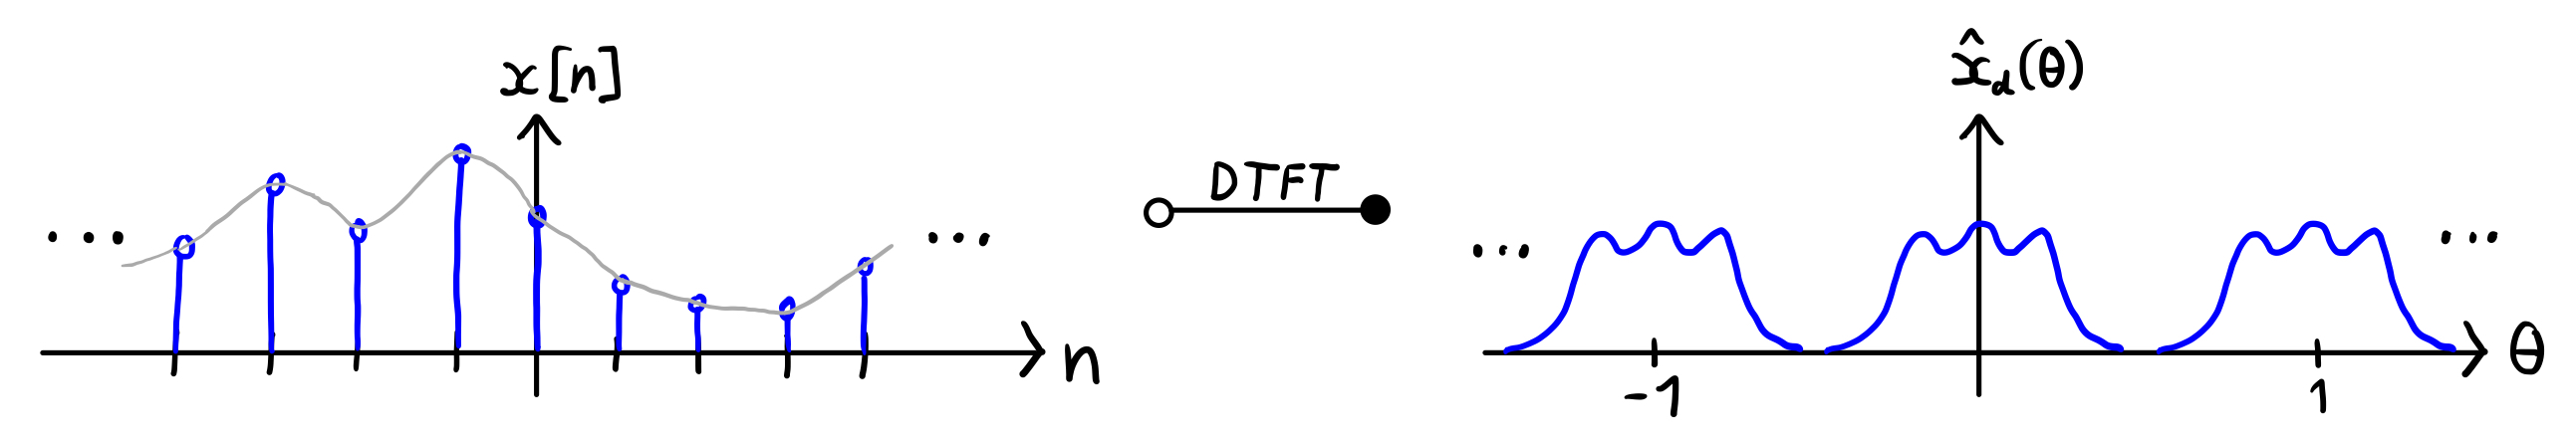
\includegraphics[width=\linewidth]{figures/dtft.jpg}
\end{frame}

\begin{frame}{DTFT: Formelsammlung}
    \begin{center}
        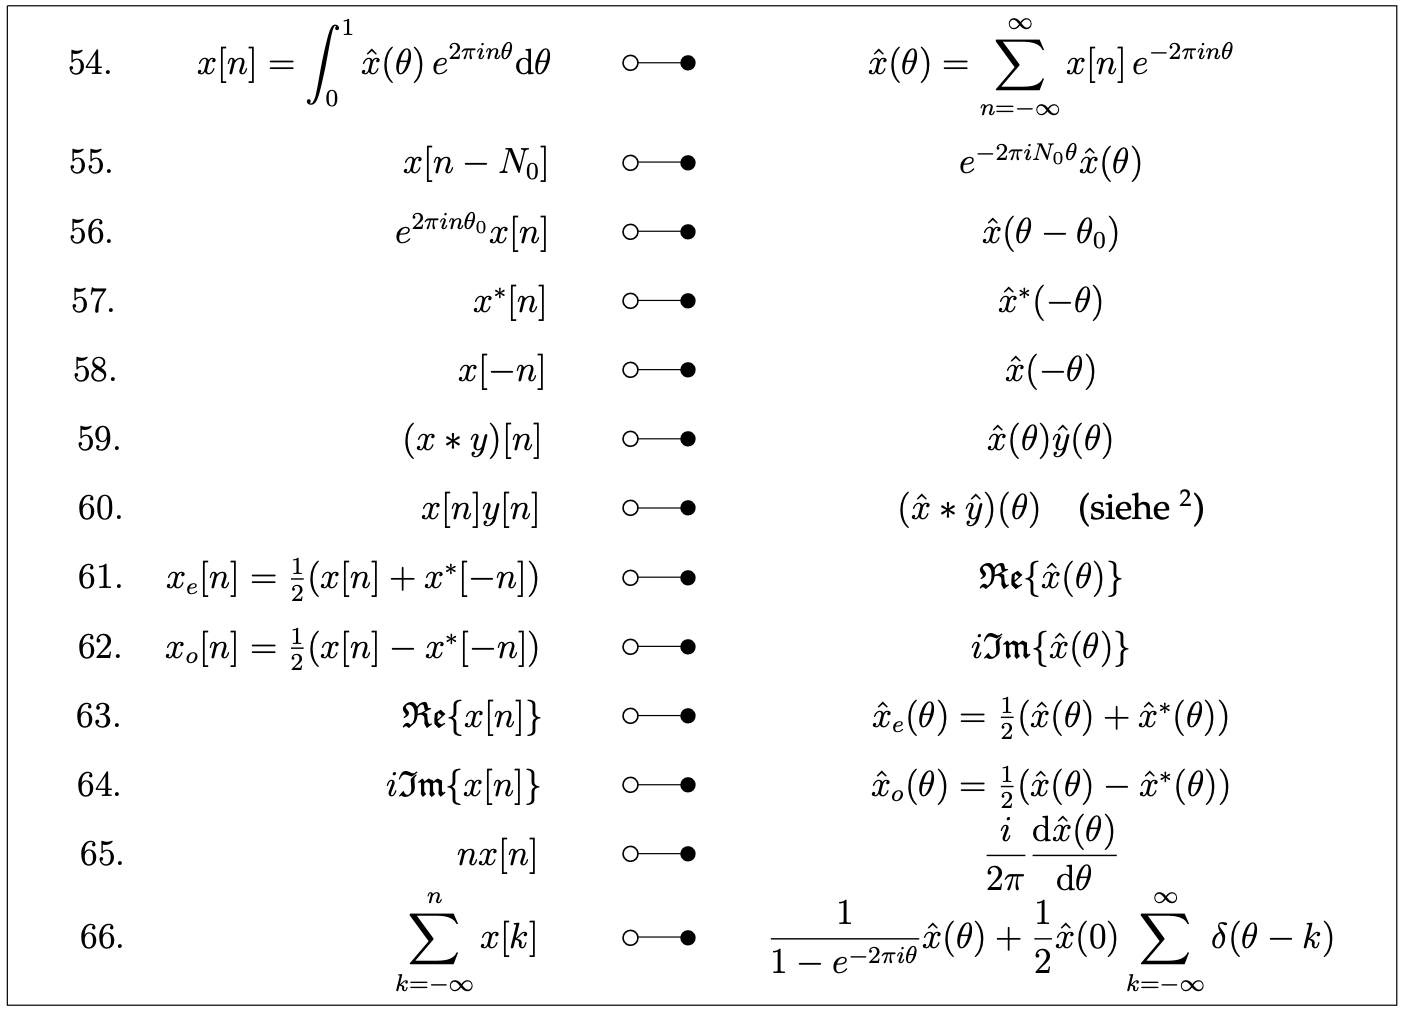
\includegraphics[width=0.7\linewidth]{figures/DTFT.png}
    \end{center}
\end{frame}

\begin{frame}{DTFT: Formelsammlung}
    \begin{center}
        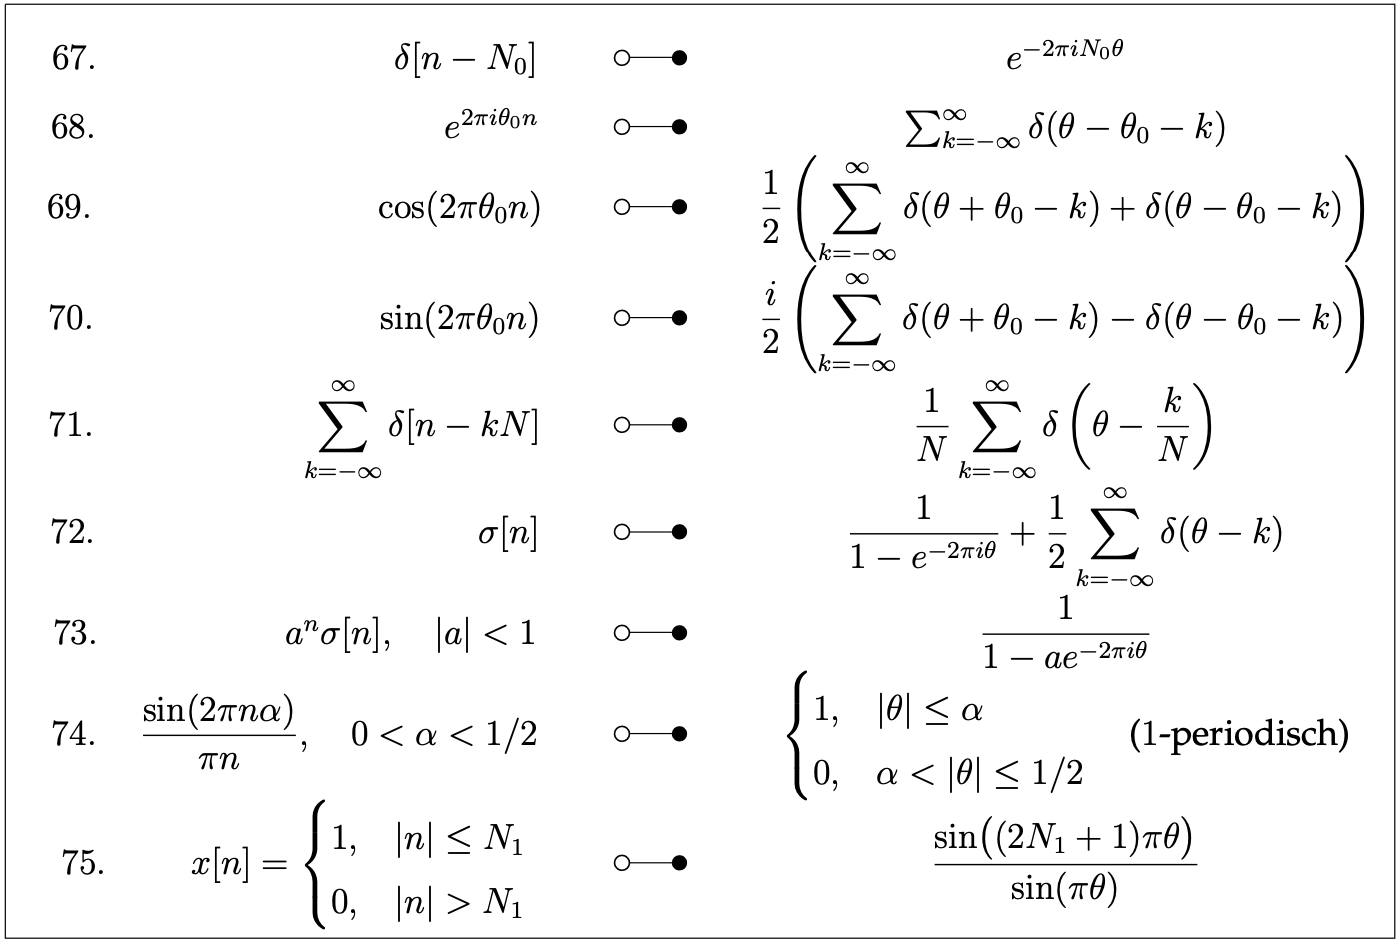
\includegraphics[width=0.7\linewidth]{figures/DTFT_paare.png}
    \end{center}
\end{frame}

\begin{frame}{Zeitdiskrete Systeme \& Eigenschaften}
    \vspace*{-0.25cm}
    \begin{center}
        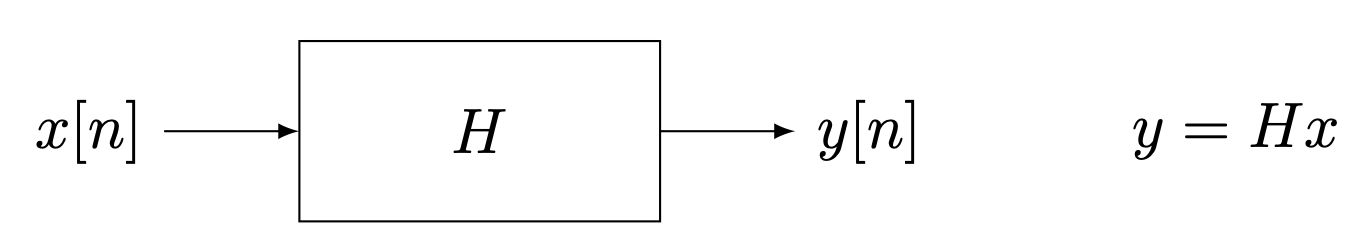
\includegraphics[width=0.6\linewidth]{figures/System_zeitdiskret.png}
    \end{center}
    \begin{itemize}
    \item \textbf{Linearität}
    \item[] $H(\alpha x_1 + x_2) = \alpha H x_1 + H x_2 \hspace{16pt} \forall x_1, x_2 \in X, \; \forall \alpha \in \mathbb{C}$
    \item[]
    \item \textbf{Zeitinvarianz}
    \item[] $H(x[\cdot -n_0]) = (Hx)[\cdot -n_0] \hspace{16pt} \forall x\in X, \; \forall n_0 \in \mathbb{Z}$
\end{itemize}
\end{frame}

\begin{frame}{Zeitdiskrete Systeme \& Eigenschaften}
    \begin{itemize}
        \item \textbf{Kausalität}
        \item[] $x_1[n] = x_2[n] \hspace{10pt} \forall n \leq n_0 \implies (Hx_1)[n] = (Hx_2)[n] \hspace{10pt} $
        \item[] $\forall n \leq n_0 \hspace{16pt} \forall x_1, x_2 \in X, \; \forall n_0 \in \mathbb{Z}$
        \item[] 
        \item \textbf{BIBO-Stabilität}
        \item[] $\forall x \in X$ mit $|x[n]| \leq B_x < \infty \hspace{10pt} \forall n \in \mathbb{Z} $
        \item[] $\implies \exists B_y < \infty$ mit $ |(Hx)[n]| \leq B_y \hspace{10pt} \forall n \in \mathbb{Z}$
    \end{itemize}
\end{frame}

\begin{frame}{Kronecker-Delta Funktion}
    Die Kronecker-Delta Funktion ist definiert als
$$\delta[n] = \begin{cases}
    1, \hspace{12pt} n = 0 \\
    0, \hspace{12pt} n \neq 0
\end{cases} \hspace{20pt} \text{bzw.} \hspace{20pt} \delta[n-n_0] = \begin{cases}
    1, \hspace{12pt} n = n_0 \\
    0, \hspace{12pt} n \neq n_0
\end{cases}$$
Es gilt $x[n] = \displaystyle\sum_{k=-\infty}^\infty x[k]\delta[n-k]$
\end{frame}

\begin{frame}{Zeitdiskrete LTI-Systeme}
    \begin{itemize}
        \item Die Systemantwort von zeitdiskreten LTI-Systemen lautet:
        \item[] $y[n] = (Hx)[n] =$
        \item[]
        \item[] 
        \item[]
        \item[] 
        \item[]
        \item[] 
        \item Die zeitdiskrete Impulsantwort ist definiert als $h[n] = (H\delta)[n]$
    \end{itemize}
\end{frame}

\begin{frame}{Zeitdiskrete LTI-Systeme}
    \begin{itemize}
    \item Die Antwort von einem LTI-System ist also:
    \item[] \fcolorbox{darkblue}{lightblue}{%
    \parbox{\dimexpr\linewidth-2\fboxsep-2\fboxrule\relax}{
    \begin{align*}
        \hspace{10pt}&y[n] = \displaystyle\sum_{k=-\infty}^\infty x[k]h[n-k] = \displaystyle\sum_{k=-\infty}^\infty x[n-k]h[k] \\
        &\underset{59}{\transform{DTFT}{1.5}}\hspace{8pt} \hat{y}(\theta) = \hat{x}(\theta)\hat{h}(\theta)
    \end{align*}
}}%
\end{itemize}
\end{frame}

\begin{frame}{Systemeigenschaften Zeitdiskreter LTI-Systeme}
    Ein LTI-System heisst ...
    \begin{itemize}
    \item[] 
    \item \textbf{kausal}, genau dann wenn:  $h[n] = 0 \hspace{10pt} \forall n < 0$
    \item[] 
    \item \textbf{BIBO-stabil}, wenn: $\displaystyle\sum_{n=-\infty}^\infty |h[n]| < \infty$, (also $h \in l^1$)
\end{itemize}
\end{frame}

\begin{frame}{Prüfungsaufgabe: Frühjahr 2017, Aufgabe 3.a)}
    
\end{frame}

\begin{frame}{Blockschaltbilder}
\begin{center}
    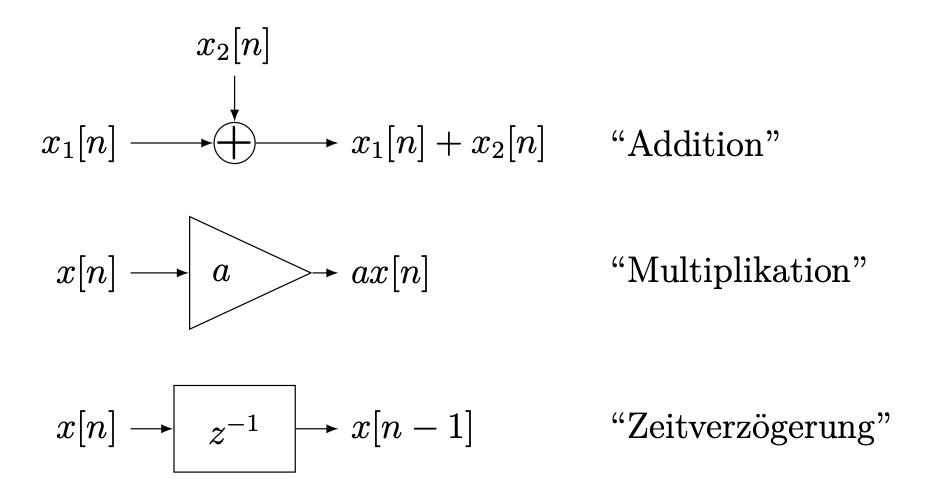
\includegraphics[width=0.9\linewidth]{figures/Blockschaltbilder.png}
\end{center}
\end{frame}

\begin{frame}{Differenzengleichungen}
    \begin{itemize}
        \item Viele zeitdiskrete LTI-Systeme lassen sich beschreiben durch:
        $$\sum_{k=0}^N a_k y[n-k] = \sum_{m=0}^M b_m x[n-m]$$
        \item Umformen dieser Gleichung ergibt:
        \begin{align*}
            &a_0 y[n] + \sum_{k=1}^N a_k y[n-k] = \sum_{m=0}^M b_m x[n-m]\\
            &\implies y[n] = -\sum_{k=1}^N \frac{a_k}{a_0}y[n-k] + \sum_{m=0}^M \frac{b_m}{a_0} x[n-m] \\
        \end{align*}
    \end{itemize}
\end{frame}

\begin{frame}{Differenzengleichungen}
    \begin{align*}
        &y[n] = -\sum_{k=1}^N \frac{a_k}{a_0}y[n-k] + \sum_{m=0}^M \frac{b_m}{a_0} x[n-m] \\
        &\text{Wir setzen } -\frac{a_k}{a_0} = \Tilde{a}_k \text{ und } \frac{b_m}{a_0} = \Tilde{b}_m \\
        &\implies y[n] = \sum_{k=1}^N \Tilde{a}_k \underset{\verticaltransform{}{0.5}{}{\hat{y}(\theta)e^{-2 \pi i k \theta}}}{y[n-k]} + \sum_{m=0}^M \Tilde{b}_m \underset{\verticaltransform{}{0.5}{}{\hat{x}(\theta)e^{-2 \pi i m \theta}}}{x[n-m]}
    \end{align*}
\end{frame}

\begin{frame}{Differenzengleichungen}
\vspace*{-0.25cm}
    \begin{center}
        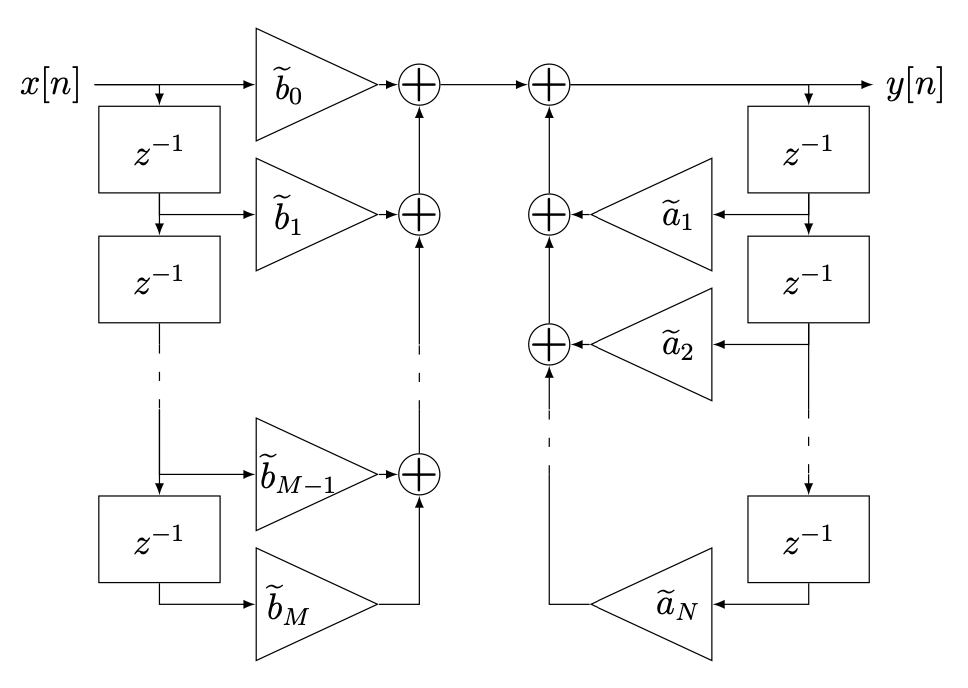
\includegraphics[width=0.55\linewidth]{figures/Blockschaltbild2.png}
    \end{center}
    \vspace*{-0.25cm}
    $$y[n] = \sum_{k=1}^N \Tilde{a}_k y[n-k] + \sum_{m=0}^M \Tilde{b}_m x[n-m]$$
\end{frame}

\begin{frame}{Differenzengleichungen: Beispiel}
    \begin{itemize}
        \item LTI-System beschrieben durch:
        $$2 y[n] - 3y[n-3] = x[n] + 6x[n-1] - 8x[n-7]$$
        \item \textbf{Ziel}: Suche $\hat{h}(\theta) = \displaystyle\frac{\hat{y}(\theta)}{\hat{x}(\theta)}$. 
        \item Es gilt: $x[n-N_0] \hspace{10pt} \displaystyle\transform{55.}{1} \hspace{10pt}\displaystyle e^{-2 \pi i N_0 \theta} \hat{x}(\theta)$
        \item DTFT auf beiden Seiten ergibt:
    \end{itemize}
\end{frame}

\begin{frame}{Differenzengleichungen: Beispiel}
    \begin{itemize}
        \item DTFT $\implies \displaystyle\left( \displaystyle\sum_{k=0}^N a_k e^{-2\pi i k \theta}\right)\hat{y}(\theta) = \displaystyle\left( \displaystyle\sum_{m=0}^M b_m e^{-2 \pi i m \theta}\right)\hat{x}(\theta)$
        \item[] 
        \item Somit $\hat{h}(\theta)= \displaystyle\frac{\hat{y}(\theta)}{\hat{x}(\theta)} = \displaystyle\frac{\displaystyle\sum_{m=0}^M b_m e^{-2 \pi i m \theta}}{ \displaystyle\sum_{k=0}^N a_k e^{-2\pi i k \theta}}
    $
    \end{itemize}
\end{frame}

\begin{frame}{FIR-Filter}
\begin{multicols}{2}
    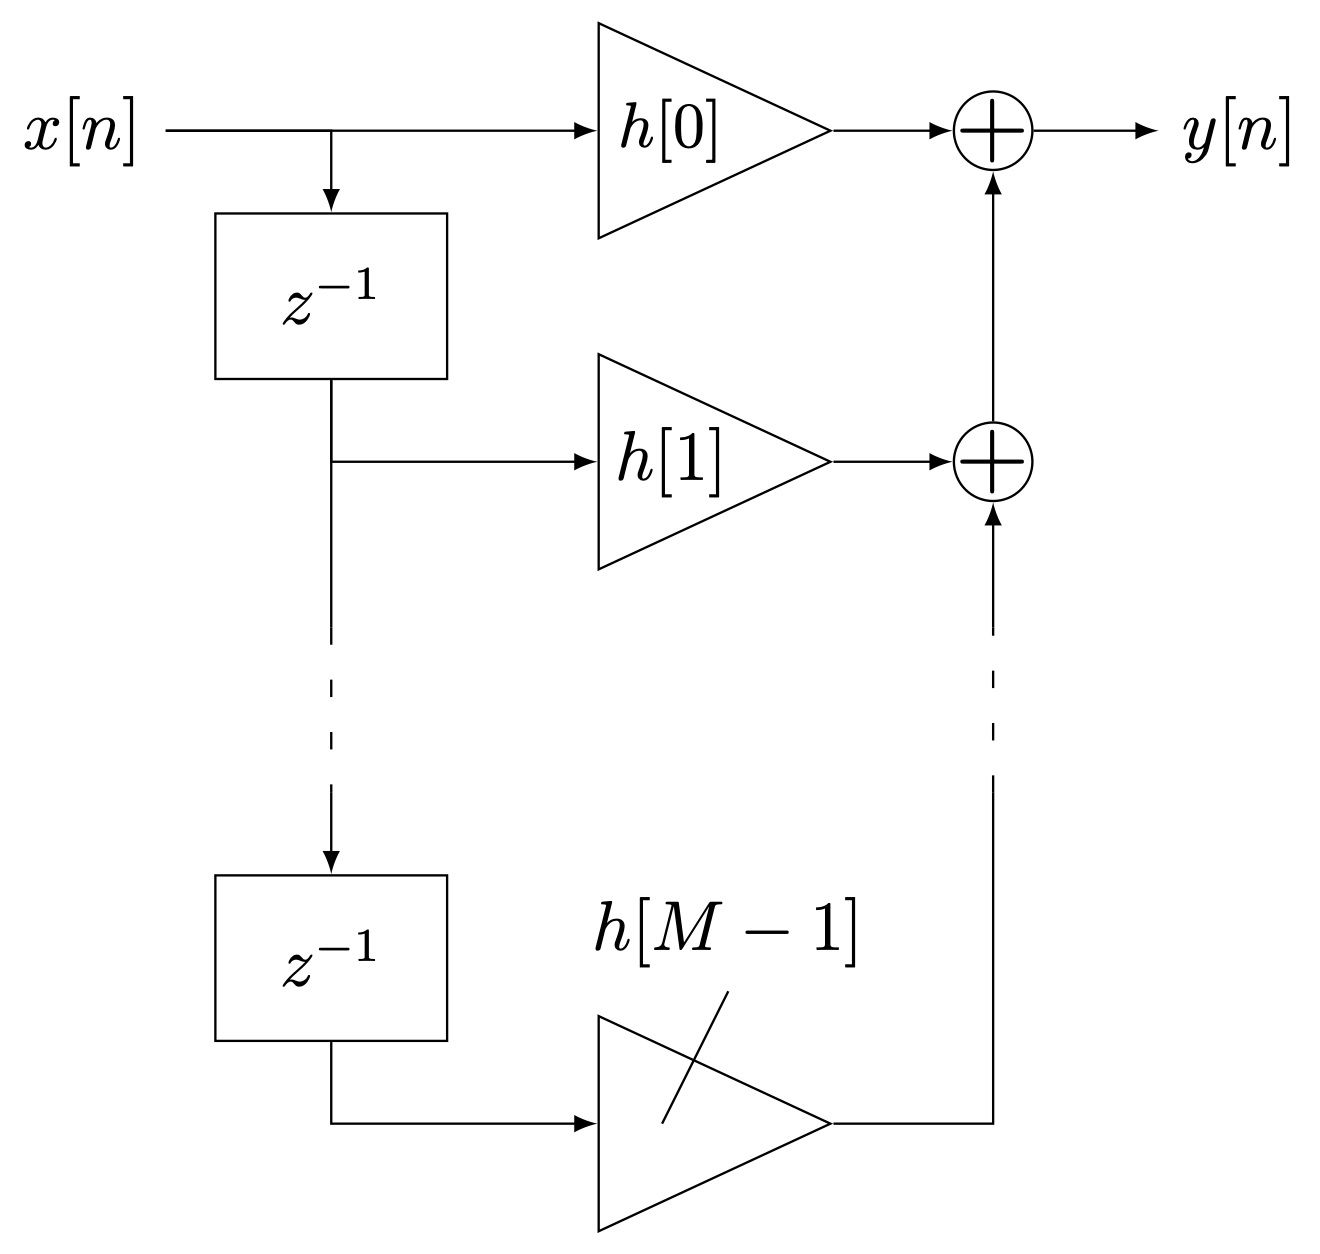
\includegraphics[width=\linewidth]{figures/FIR.png}

    \vfill \null
    \columnbreak

    \begin{itemize}
        \item Impulsantwort hat \textbf{endliche Länge}
        \item FIR-Filter haben keine Rückkopplungen
    \end{itemize}
    \vspace*{-0.5cm}
    \begin{align*}
        y[n] \overset{\text{LTI}}{=} &\sum_{l=-\infty}^\infty h[l] x[n-l] \\
        = &\sum_{l=0}^{M-1} h[l]x[n-l] 
    \end{align*}
\end{multicols}
\end{frame}

\begin{frame}{IIR-Filter}
    Die Impulsantwort von IIR-Filtern hat \textbf{unendliche Länge}. Das Blockschaltbild hat Rückkopplungen $\implies$ oft Stabilitätsproblemen\\
    \begin{center}
        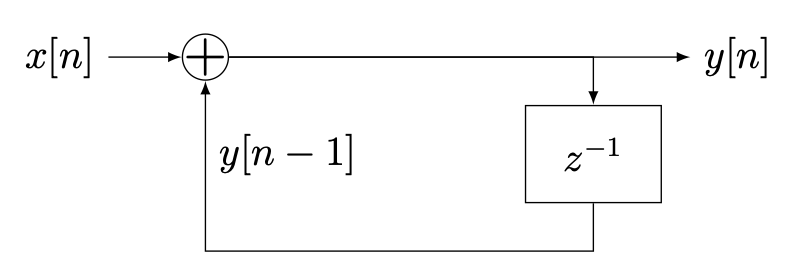
\includegraphics[width=0.8\linewidth]{figures/IIR.png}
    \end{center}
\end{frame}

\begin{frame}{IIR-Filter}
\begin{center}
        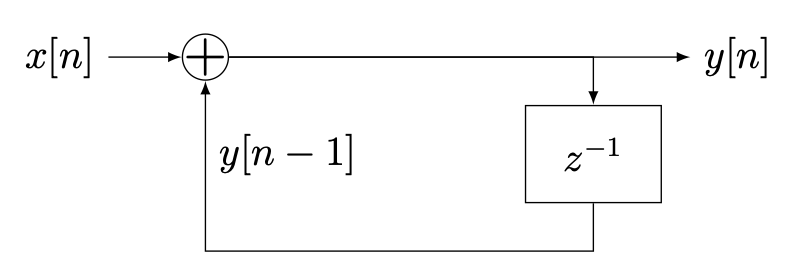
\includegraphics[width=0.4\linewidth]{figures/IIR.png}
    \end{center}
    \vspace*{-0.5cm}
    \begin{align*}
        y[n] &= x[n] + y[n-1] = x[n] + \sum_{k=-\infty}^{n-1}x[k] \\
        &= \sum_{k=-\infty}^n x[k] \overset{\text{LTI}}{=} \sum_{k=-\infty}^\infty x[k]h[n-k]
    \end{align*}
    $$\implies h[n-k] = \sigma[n-k] \Leftrightarrow h[n] = \sigma[n]$$
\end{frame}

\begin{frame}{Prüfungsaufgabe: Frühjahr 2017, Aufgabe 3.b)}
    
\end{frame}

\end{document}
